\section{Method}
\label{sec:method}

% Fig. 1 (pipeline) \todo{draw: situation -> codebook candidates -> safety filter -> style features -> A/B queries (EUBO) -> theta -> executed path}

\subsection{Problem setting}
In a situation $s$ the robot knows its own state (speed, two past positions), its destination and the positions and velocities of
nearby people. A user has a preference over how the robot walks, which we model as a linear utility over style features.
The user answers a small number of A/B questions in a few query situations; the robot must then choose its path in new situations
the user was never asked about.

\subsection{Walking-behaviour codebook}
\label{sec:candidates}
A VQ-VAE~\citep{vandenoord2017neural} with $K=16$ codes is trained on pedestrian futures expressed in the heading frame as deviations
from constant velocity (6 points every 0.8\,s, 4.8\,s). Decoding every code from the robot's current speed gives $K$ candidate paths.
A prior network $p(\text{code} \mid s)$, trained on the same data with the destination and a summary of nearby people as input,
scores how typical each candidate is for a person in that situation.
\todo{training details: data split by person, epochs, prior inputs; GC: 12,159 test conflict situations; ETH/UCY: 590}

\paragraph{Safety filter.}
People are extrapolated at constant velocity; a candidate is safe if its minimum distance to everyone is at least $c=0.5$\,m and its
progress towards the destination is at least $\rho=0.5$ times the best candidate's. The preference only chooses among safe candidates:
\begin{equation}
  \mathcal{C}(s) = \bigl\{ k \;:\; d_{\min}(s,k) \ge c,\; \mathrm{prog}(s,k) \ge \rho \max_{k'} \mathrm{prog}(s,k') \bigr\}.
\end{equation}

\subsection{Style features}
Each safe candidate is described by $\phi(s,k) \in \mathbb{R}^5$, none of which has an a-priori right sign:
\emph{side} ($\tanh$ of the lateral offset from the conflict person at closest approach),
\emph{front} (crossing ahead of or behind them), \emph{yield} (mean speed relative to the current speed),
\emph{detour} (largest deviation from the straight line to the destination) and \emph{human} ($\log p(\text{code}\mid s)$).
Features are standardized over the safe candidates of the query situations.

\subsection{Preference learning and query selection}
\label{sec:preference}
The user's utility is $u(s,k) = \theta^\top \phi(s,k)$. Answers follow the Bradley--Terry model~\citep{bradley1952rank}
$P(i \succ j \mid \theta) = \sigma(\theta^\top(\phi_i - \phi_j))$ with prior $\theta \sim \mathcal{N}(0, I)$; the posterior is
approximated by a Laplace approximation (Newton's method for the MAP, inverse Hessian as covariance).
Each query asks the pair maximizing the expected utility of the best option~\citep{astudillo2023qeubo},
\begin{equation}
  (i,j) = \operatorname*{arg\,max}_{i \ne j} \; \mathbb{E}_{\theta \sim p(\theta \mid \mathcal{D})}\bigl[\max\{u_i, u_j\}\bigr],
\end{equation}
estimated with 512 posterior samples. At test time the robot executes
$\hat k_n(s) = \arg\max_{k \in \mathcal{C}(s)} \hat\theta_n^\top \phi(s,k)$ with $\hat\theta_n$ the posterior mean after $n$ answers.

% Formal regret definition (11/18 feedback item 4). Setting, safe set and executed path are defined in Sec. 3.
\subsection{Evaluation: simple regret}
\label{sec:regret}

\paragraph{Users.}
For evaluation a user is a unit vector $\theta^\ast$ ($\lVert\theta^\ast\rVert = 1$) with utility $u^\ast(s,k) = \theta^{\ast\top}\phi(s,k)$,
who answers a question $(i,j)$ with $P(i \succ j) = \sigma\bigl(\beta\,(u^\ast(s,i) - u^\ast(s,j))\bigr)$, $\beta = 5$.
After $n$ answers a method returns $\hat\theta_n$ (the Laplace posterior mean for Bradley--Terry methods, the DPO solution for DPO,
Sec.~\ref{sec:dpo}) and executes $\hat k_n(s)$ of Eq.~\eqref{eq:exec} among the safe candidates $\mathcal{C}(s)$ of Eq.~\eqref{eq:safe}.

\paragraph{Simple regret.}
The regret of that choice is the utility lost against the user's best safe candidate,
normalized by the utility range of the situation so that situations are comparable:
\begin{equation}
  r_n(s) = \frac{\max_{k \in \mathcal{C}(s)} u^\ast(s,k) \;-\; u^\ast\bigl(s,\hat k_n(s)\bigr)}
                {\max_{k \in \mathcal{C}(s)} u^\ast(s,k) \;-\; \min_{k \in \mathcal{C}(s)} u^\ast(s,k)}
  \;\in [0,1].
  \label{eq:regret}
\end{equation}
The reported number is its expectation over users and held-out test situations,
\begin{equation}
  \mathrm{SR}_n = \mathbb{E}_{\theta^\ast}\Bigl[\frac{1}{|\mathcal{S}_{\text{test}}|}
  \sum_{s \in \mathcal{S}_{\text{test}}} r_n(s)\Bigr],
  \label{eq:sr}
\end{equation}
where answers are only collected in query situations disjoint from the test situations
($\mathcal{S}_{\text{query}} \cap \mathcal{S}_{\text{test}} = \emptyset$; sizes in Sec.~\ref{sec:experiments}).
$\mathrm{SR}_n = 0$ for the oracle ($\hat\theta = \theta^\ast$);
a uniformly random safe candidate gives $\mathrm{SR} \approx 0.5$.

\paragraph{Why simple regret.}
Queries cost the user's attention but no driving utility, and what matters is the path the robot
executes afterwards. The objective is therefore best-arm identification (simple regret) rather
than cumulative regret over the queries. EUBO~\citep{astudillo2023qeubo} is one-step Bayes-optimal
for exactly this objective under noise-free answers, which motivates its use.
Fig.~\ref{fig:regret} plots $\mathrm{SR}_n$ against the number of queries $n \in \{0,2,5,10,20\}$.

\paragraph{Variants used elsewhere.}
\emph{Closed loop:} at every 0.8\,s re-planning step $t$ of a drive, Eq.~\eqref{eq:regret} is evaluated
on that step's safe set $\mathcal{C}(s_t)$ and averaged over the steps of the episode (step regret).
\emph{Candidate generators:} to compare two generators $A$ and $B$ on the same situation, the max and min
in Eq.~\eqref{eq:regret} are taken over $\mathcal{C}_A(s) \cup \mathcal{C}_B(s)$ (union regret), so a generator
whose candidates miss what the user wants is penalized even when it picks its own best;
the per-generator regret of Eq.~\eqref{eq:regret} is not comparable across generators.
\emph{Pilot:} with real participants $\theta^\ast$ is unknown; the measurable proxy is the share of
held-out (test-block) answers that $\hat\theta$ predicts.

% Figure (utils/plot_regret_curves.py -> reports/fig_regret.pdf)
\begin{figure}[t]
  \centering
  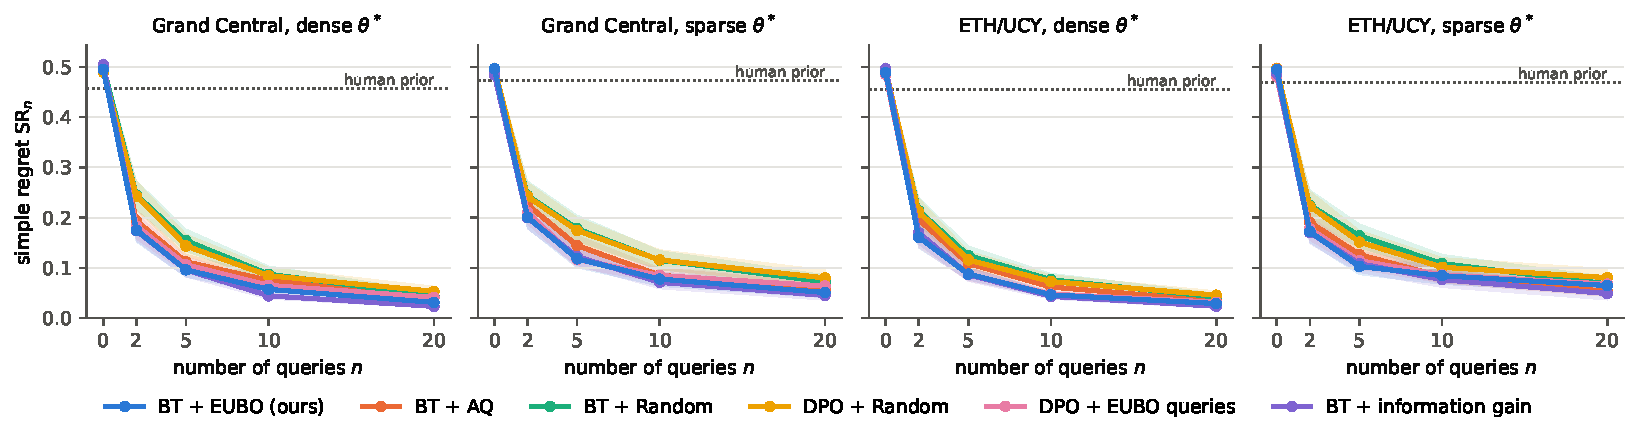
\includegraphics[width=\linewidth]{figures/fig_regret.pdf}
  \caption{Simple regret $\mathrm{SR}_n$ (Eq.~\ref{eq:sr}) on held-out situations against the number of
  A/B queries. Shaded: 95\% bootstrap CI over 200 synthetic users. Dotted: human prior only; the oracle is 0. BT: Bradley--Terry (Laplace); DPO: Sec.~\ref{sec:dpo}.}
  \label{fig:regret}
\end{figure}

